
\documentclass[preprint]{elsarticle}

\usepackage{amsmath}
\usepackage{amsfonts}
\usepackage{amssymb}
\usepackage{url}
%\usepackage{cite}
\usepackage{float}
\usepackage{lipsum}
\usepackage{caption}
\usepackage{graphicx}
\usepackage{color}
\usepackage{listings}
\usepackage{stmaryrd}
\usepackage[ruled, vlined, linesnumbered]{algorithm2e}
\usepackage{listings}
\usepackage{booktabs}
\usepackage{relsize}
\usepackage{multicol}
\usepackage{cancel}
\usepackage{wrapfig}
\usepackage{todonotes}
\usepackage{natbib}

\lstset{language=C}

%\newtheorem{claim}{Claim}
\newtheorem{definition}{Definition}
\newtheorem{theorem}{Theorem}
% \newtheorem{corollary}{Corollary}
% \newtheorem{example}{Example}
% \newtheorem{observation}{Observation}
% \newtheorem{definition}{Definition}
\newtheorem{instance}{Instance}
\newtheorem{observation}{Observation}
 
\graphicspath{{figs/}}
\newcommand\tuple[1]{\langle #1 \rangle}


\pagestyle{plain}
\pagenumbering{arabic}



\makeatletter
\newenvironment{Ualgorithm}[1][H]
  { \def\@algocf@capt@plain{top}% 
    \begin{algorithm}[#1]}
  {\end{algorithm}}
\makeatother

\usepackage{etoolbox}
\makeatletter
\pretocmd\start@align{%
  \if@minipage\kern-\topskip\kern-\abovedisplayskip\fi
}{}{}
\makeatother

\makeatletter
\newcommand{\removelatexerror}{\let\@latex@error\@gobble}
\makeatother


\begin{document}
\begin{center}

\textbf{Submission to Information Sciences Special Issue on Dependability in Parallel and Distributed Systems and Applications}
\end{center}


\noindent Dear Guest Editors, \\

We would like to submit the following manuscript entitled
``A Performance Comparison of Algorithms for Byzantine
Agreement in Distributed Systems'' for publication review for the 
Special Issue on Dependability in Parallel and Distributed Systems and Applications.

The Byzantine Agreement problem aims to achieve reliability in consensus
protocols despite the failure of some number of components.  
Analysis of algorithms under varying parameters and practical constraints through experimental evaluation can be key to understanding the performance and trade-offs of theoretically well-performing algorithms.

We focus on implementation and analysis of three performant Byzantine
Agreement algorithms with best results for their respective objectives of
optimizing only communication complexity or latency, or meeting the
worst-case bounds on both.

Our experimental analysis shows that the algorithms perform differently for different network sizes.
For networks with strict bandwidth constraints, algorithm by
Braud-Santoni et al.~\cite{BGH13} allows high flexibility in changing the size
of the network. For high variance of fault ratios, algorithm by Ben-Or et al.
\cite{BPV06} prevented byzantine processes from influencing the communication
complexity. Comparison of elapsed real time and CPU time utilization provides
better insight into the utility of one of the parallel algorithms.  Moreover,
we make modifications to the algorithm by Kowalski et al. \cite{KM13} to
improve the communication bits sent in every round of the protocol.

Quantifying the performance of the algorithms empirically provides a practical
understanding and insight into how the different algorithms perform under different
conditions to achieve consensus in distributed systems.

Thank you. \\

\noindent Sincerely,

\noindent Shreya Agrawal and Khuzaima Daudjee 

\noindent University of Waterloo

%%%%%%%%%%%%%%%%%%%%%%%%%%%%%%%%%%%%%
%We focus on implementation and analysis of three recently proposed algorithms with best algorithms for their respective agendas---(1) algorithm \textit{Quorum} by Ben-Or et al. \cite{BPV06}, (2) algorithm \textit{Pull-Push} by Braud-Santoni et al.~\cite{BGH13}, and (3) algorithm \textit{EIG} (Exponential Information Gathering) by Kowalski et al. \cite{KM13}. 
%In general, the randomized algorithm \textit{Pull-Push} performs better than
%the other two in terms of communication complexity. When latency is considered,
%algorithm \textit{Quorum} performs better.
%
%In the case of a small network, with the number of processes less than $32$ and
%a low fault percentage---(approximately less than $10\%$), algorithm
%\textit{EIG} performs better since it considers the number of faults in its
%protocol. However, its performance degrades under high fault ratio. We show
%that under high variance of network size over time if the increase in size is
%within the next power of $2$, then for algorithm \textit{Pull-Push} the number
%of bits sent per node remains the same. For networks with strict bandwidth
%constraints, this allows high flexibility in changing the size of the
%network. For high variance of fault ratios, algorithm \textit{Quorum} prevented
%byzantine processes from influencing the communication complexity. Moreover,
%we improve upon the results obtained for algorithm \textit{EIG} by making
%certain changes in the algorithm itself---removing the redundant information
%being sent in every round regarding the list of byzantine nodes. This further
%%improves the number of bits sent in every round of the protocol.

\newpage
\title{A Performance Comparison of Algorithms for Byzantine Agreement in Distributed Systems \\ {\large Paper ID 67} \vspace{-1cm}}

%\author{\IEEEauthorblockN{Paper ID 67}}

%\author{
%\IEEEauthorblockN{Shreya Agrawal}
%\IEEEauthorblockA{School of Computer Science\\
%University of Waterloo\\
%s8agrawa@uwaterloo.ca }
%
%\and
%\IEEEauthorblockN{Khuzaima Daudjee}
%\IEEEauthorblockA{School of Computer Science\\
%University of Waterloo\\
%kdaudjee@cs.uwaterloo.ca }}

\maketitle


\begin{abstract}

Ensuring that all processes in a network agree in the
presence of byzantine processes is known to be a challenging task in
distributed systems. This is fundamentally due to two reasons: (1)
asynchronous execution of systems, and (2) byzantine
processes colluding together to inject arbitrary values in a synchronous/asynchronous
system. These issues pose a problem to scalability, safety, liveness,
reliability and performance of the system. Impossibility results have
been shown for deterministic solutions for the first case, even in the
presence of one fault. For the second case, researchers have taken
different approaches to find performant solutions. While strong
theoretical results give us an insight into the efficiency of an
algorithm, they sometimes come with large hidden constants and might not
be practical for a real system. In this paper, we compare the 
performance of two randomized algorithms, one using the {\em pull-push} approach
and the other using the concept of {\em quorums}, and a third recent simple
deterministic algorithm that we expect to perform 
better in certain cases.
Three metrics have been used for comparison - {\em bit}
complexity, {\em round} complexity and {\em latency} with respect to varying network sizes and
faulty processes. By implementing a testbed environment and using these metrics, we identify instances for which each 
algorithm performs differently under varying resource constraints and
number of faults. We show that for small networks ($n<32$) and up to $10\%$ of faulty processes, the simple deterministic algorithm performs better than any of the randomized ones. However, for larger networks, the best performance is shown by the algorithm with the pull-push approach. Although, the trade-off here is between communication and round complexity, the second randomized algorithm performs much better in terms of round complexity than the other two. 

\end{abstract}

\noindent {\bf Keywords:} Distributed systems, Performance, Byzantine failures, Fault-tolerant, Consensus, Complexity.

\section{Introduction}

The Distributed Consensus problem, introduced in 1980 by Pease et al. \cite{PeaseSL80}, is one of the most important and well-studied problems in distributed systems. In essence, the problem deals with multiple processes, each with an opinion initially, cooperating with each other to reach an agreement. The motivation for this problem arises from cases such as database transactions, where a number of systems need to agree on whether to commit or abort a transaction, or in aircraft controllers that need to agree on which plane should take-off or land first. In the latter case, in a safety-critical system such as this one, it is essential that aircraft controllers reach an agreement within a bounded period of time and all the controllers have the same decision, while in the former case, it is necessary that the systems eventually reach an agreement. Therefore, any consensus reaching algorithm needs to satisfy certain correctness conditions that are formally given as follows \cite{PeaseSL80}:

\begin{itemize}
    \item \textit{Consistency}: All processes agree on the same value and all the decisions are final.
    \item \textit{Validity}: If all processes start with the same initial value $v$, then $v$ is the only allowable decision for all processes.
    \item \textit{Termination}: All processes reach a decision.
\end{itemize}

%TODO: give example of synchronous

These conditions also define the safety and liveness conditions that a distributed consensus algorithm must satisfy.  The \textit{consistency} and \textit{validity} condition is a safety condition, and safety will be violated if any two processes decide on different values. The \textit{termination} condition specifies the liveness condition of the system. For a system to continue executing correctly until it terminates, all processes must eventually come to a conclusion.

In real-world applications, it would be unrealistic to assume that the systems involved in solving the problem will continue to work correctly, for the whole duration, as specified by the protocol. There may be cases such as when the communication links between systems break and the system \textit{partitions}, the network becomes congested due to too many requests, or the messages are not delivered in order. To achieve reliability in distributed systems, protocols are needed which enable the system as a whole to continue to function despite the failure of a limited number of components. Another challenge that real-world systems face is the problem of \textit{asynchronous} execution, in which different components might face arbitrary, unbounded delays. It was shown in a well-known result by Fischer et al. \cite{FischerLP83} that reaching distributed consensus deterministically becomes impossible in an asynchronous system with just one faulty process. It becomes difficult to differentiate a process that has failed from a process that is simply slow in responding. Components cannot execute in a lock-step manner since there does not exist a global clock. The asynchronous model is strictly harder than the synchronous model. 

It was shown in \cite{LamportSP82} that consensus can never be reached even between two processes if there is a link failure. Under the assumption that the links do not display any kind of fault, one needs to analyze scenarios in the case of process failures. Generally, the kind of failures that a process can encounter is either a \textit{fail-stop} failure or a \textit{Byzantine failure}. Fail-stop failures occur when processes fail by stopping. In the case of a byzantine failure, the processes fail by acting maliciously. Depending on the ratio of faulty processes to all the processes, consensus may be impossible even when the system is synchronous. The problem of solving consensus in the presence of byzantine failures came to be known as the Byzantine Agreement problem \cite{LamportSP82}. With the increasing number of malicious attacks reported in recent times and software bugs leading processes behaving aribitrarily, dealing with this problem has become more important than ever before.

A vast amount of work has been done over the years to solve the Byzantine Agreement problem, and different approaches have been taken for various models of the problem. Randomized algorithms allowed us to overcome the barrier of the impossibility result in the asynchronous setting. Even in the synchronous setting, they provided major improvements over the deterministic algorithms by a factor polynomial in the size of the network. The probabilistic techniques provide an advantage - they allow us to eliminate the worst-case scenarios by giving them a probability of $0$ and a probability distribution is given in the other cases. While the literature is rich in theoretical results, there has been a lack of extensive practical results for the proposed algorithms. This can be largely attributed to the fact that simple algorithms are theoretically inefficient, while the more complex ones are hard to implement. Theoretical results give us information about the worst case scenarios, although practically, the system does not always run in the worst case. It would also be unrealistic to completely relax this assumption. Analysis techniques using the Big `O' notation sometimes hide away large constants which are of significance when we look at memory or bandwidth consumption in a real-world application. Many complex algorithms make certain assumptions about systems, for example, the existence of a large fraction of faulty processes. Whereas, there may actually be only a small fraction of faulty processes and in such cases the algorithm would be unnecessarily complex and inefficient.

Motivated by the need to analyze algorithms under such varying conditions, we evaluate the performance of three recently proposed solutions for the Byzantine Agreement problem. Two of these are randomized algorithms - (1) by Ben-Or et al. \cite{BPV06}, which we call algorithm \textit{Quorum} throughout the paper, and (2) an almost-everywhere to everywhere algorithm by Braud-Santoni et al. \cite{BGH13} with the almost-everywhere algorithm of \cite{KSSV06}, which we call algorithm \textit{Pull-Push}. An almost-everywhere algorithm reaches consensus among all but a fraction of the processes and an almost-everywhere to everywhere algorithm reaches consensus among all the processes when an almost-everywhere consensus exists. The third is a deterministic algorithm, due to Kowalski et al. \cite{KM13}, which we refer to as algorithm \textit{EIG}. We vary two parameters to define the workload of the system - the number of processes, and with that the fraction of faults in the system. For evaluation, we use three metrics, two of which are commonly used for theoretical evaluation - communication complexity and round complexity, and the other one being latency. We report on the behavior of the algorithms on varying the parameters and their effects on these metrics. 

The algorithm \textit{Pull-Push}, is one of the most recent and best known performing result in terms of communication complexity. The main contribution of the paper has been to give an almost-everywhere to everywhere solution, which improves the amortized communication complexity to $\tilde{O}(1)$ per node\footnote{$\tilde{O}$ is same as $O$ up to a poly-logarithmic factor}. The previously best known result was $\tilde{O}(n^{1/2})$ given by \cite{KLST11}. The algorithm uses the model previously considered in \cite{KLST11,KSSV06,BPV06,KS09}, that of a synchronous, full-information model, with a non-adaptive adversary. They also show that similar results can be shown even in the case of an asynchronous model. Even though, the communication complexity result is the best known, there has been a trade-off with round complexity which is poly-logarithmic in the size of the network. This trade-off between communication and round complexity motivated us to pick the algorithm \textit{quorum} for comparison. Algorithm \textit{quorum}, due to Ben-Or et al., has a round complexity of $O(logn)$ although it shows a quasi-polynomial communication complexity of $n^{O(logn)}$. It uses the same setting as \textit{Pull-Push} and makes use of the well-known Feige's protocol of collective coin-flipping to decide on a small committee with the same fraction of good processes as in the whole network, which then runs a leader election protocol for agreement. While both these randomized algorithms attempt to improve upon the metrics for performance comparison, they consider worst-case scenarios when the fraction of adversarial processes is $n/3$ and $n/4$, respectively. On the other hand, in a real-world system, this fraction might actually be really small. This motivated us to choose a deterministic algorithm for comparison which considers this fraction during the execution of its algorithm and thus provides much better results for both communication and round complexity when the number of adversarial nodes to the size of the network is really small. These experimental results will allow us to determine the most relevant algorithms to pick given the workload and requirements of a system, i.e., the fraction of adversarial nodes, the bandwidth requirements and latency. 


Section~\ref{sec:background} gives an introduction to the various models used to solve distributed consensus problem and provides a summary of related work in this field over the years. In Section~\ref{sec:algos}, we elaborate on the three algorithms under comparison. Section~\ref{sec:eval} and \ref{sec:results} details the implementation and evaluates the results obtained from the experiments. This is followed by a discussion and conclusion in Section~\ref{sec:conc}.

%TODO: 1) Consensus problem
%    2) With faults - different kind of faults -> there repercussions
%    3) Why is byzantine failures important (motivate the problem)
%
%TODO: Why so many algorithms in this area? What difference is there? Why study more? Why do a survey? Different kind of algorithms - Deterministic, randomized, almost everywhere
%
%TODO: What am I doing? What am I trying to find out? Give outline of paper
%
%ACID
%
%reliability, consistency, availability
%
%SAFETY and LIVENESS
%
%
%TODO: Give example - Alice and Bob? - show violation of above three








\section{Background}
\label{sec:background}

\subsection{Problem statement}
The problem of Byzantine Agreement, in its most basic form is defined as follows \cite{PeaseSL80}:

\begin{definition}
    Let $\mathcal{P}$ be a protocol among $n$ processes $P = \{ P_1, P_2, \dots, P_n\}$, such that $B \subset P$ processes are byzantine. Each process $P_i$ starts with an input bit $b_i$, and $P_i$ outputs a bit $c_i$ at the end of the protocol. $\mathcal{P}$ is a Byzantine Agreement Protocol, if the following conditions hold:
\begin{itemize}
    \item \textit{Consistency}: For any two non-faulty processes $P_i$ and $P_j \in P \backslash B$, $c_i = c_j$.
    \item \textit{Validity}: If $b_i = b$ for all non-faulty processes $P_i \in P \backslash B$, then $c_i = b$ for all non-faulty processes $P_i$.
    \item \textit{Termination}: Protocol $\mathcal{P}$ terminates with probability $1$.
\end{itemize}
\end{definition}

A protocol is said to be $k$-fault tolerant if it operates correctly as long as no more than $k$ processes fail during execution. The following theorem by \cite{LamportSP82,PeaseSL80} shows the impossibility result when $k \geq n/3$.

\begin{theorem}
There is a $k$-fault tolerant synchronous protocol to solve the byzantine agreement problem iff $k < n/3$.
\end{theorem}

\subsection{Complexity measures}

The practicality of agreement protocols depends heavily on their computational complexity. Theoretically, when talking about complexity measures of algorithms for distributed consensus, one generally uses the following two metrics:
\begin{itemize}
\item \textit{Round} complexity - the number of rounds of message exchange before all the non-faulty processes decide.
\item \textit{Communication} complexity - the total number of messages sent per process or the total number of bits sent per process.
\end{itemize}
For empirical analysis, we also consider the following metric: 
\begin{itemize}
\item \textit{Latency} - the overall CPU time utilization or elapsed real time from start till all the non-faulty processes decide.
%\item \textit{Memory} comsumption, is the memory requirement for the execution of an alorithm for a configuration and depends mainly upon the data structures used for storing of values.
\end{itemize}
%All of these quantities are in general dependent on which faults occur and when, and how parallel the algorithm is. As the size of the system increases, i.e., the number of processes increase, the expected number of faults grows linearly with it. Also, for example, a highly parallel system might require more memory but reduces the round complexity. Round complexity is also an indication of how much of the algorithm can be executed in parallel.

\subsection{Previous work}

\subsubsection{Deterministic Solutions}
Fischer and Lynch \cite{Fischer81alower} proved that $k + 1$ is the round
complexity in the worst case for a $k$-fault tolerant synchronous protocol. If
the messages were not \textit{authenticated}, the message complexity was
initially shown to be exponential in the number of process by Pease et
al.~\cite{PeaseSL80}. In 1998, Garay and Moses \cite{GarayM98}, with
modifications to the two phase protocol of Bar-Noy et al.~\cite{BDDS87} using
the EIG data structure, improved the message complexity further to polynomial
time. If authenticated messages were sent, Dolev and Reischuk \cite{DolevR85},
proposed an algorithm using $O(n + k^2)$ messages. In an attempt to lower the
communication costs, researchers either lowered the fraction of faulty
processes to a smaller number \cite{DRS90} or increased the maximum number of
rounds needed in the worst case \cite{TPS87}. It was only recently that
Kowalski et al. \cite{KM13} proposed a simple algorithm that holds for the
optimal range and optimal number of communication rounds while lowering the
communication complexity to $O(n^{3}logn)$.

\subsubsection{Randomized Solutions} Probabilistic solutions were proposed to
circumvent the lower bounds on round and message complexity imposed by
deterministic settings. They used the idea of a common coin which was seen as
`sufficiently random' by `sufficiently many' random processes.  In the
asynchronous setting, using randomized algorithms, Ben-Or \cite{Ben-Or83}
showed that if $k < n/5$, then consensus is achievable with probability $1$.
Rabin \cite{Rabin83} showed constant expected round complexity if $k < n/4$.
Greatly improved results have been shown in \cite{PCR14, KKKSS08, MHR14} for
non-adaptive adversary and in \cite{KS13,AAKS14} for an adaptive adversary.
Assuming that communication channels are \textit{private} between every pair of
processes, the algorithm proposed by Patra et al.~\cite{PR10} shows constant
expected round complexity and $\tilde{O}(n^2)$ message complexity. These bounds
are also applicable to the asynchronous setting. Holtby et al.~\cite{HKK08} 
proved an $\Omega(\sqrt[3]{n})$ lower bound on both message complexity and
round complexity for synchronous systems, under restrictive assumptions.

\subsubsection{Almost-Everywhere Solutions} The almost-everywhere byzantine
agreement problem was introduced by Dwork et al.~\cite{DPPU88}. It is
a relaxed version of the byzantine agreement problem and requires all but
$O(log^{-1}n)$ fraction of the processes to agree on a common output. For the
algorithm by King et al.~\cite{KSSV06}, the round and message complexities are shown to be
poly-logarithmic in $n$. Construction of byzantine agreement from
almost-everywhere byzantine agreement, called almost-everywhere reduction, was
proposed in \cite{KS09,KLST11}, using $\tilde{O}(\sqrt{n})$ bits per process
and poly-logarithmic number of rounds.  Papers such as those by King et al.~\cite{KLST11} used
push-pull protocols, the complexity of which is dictated by the complexity of
the first \textit{push} phase and the size of the candidate lists, i.e., the
number of all possible outputs. Braud-Santoni et al.~\cite{BGH13} propose an
almost-everywhere to everywhere solution using the almost-everywhere algorithm
by King et al.~\cite{KSSV06}.

%\begin{table}[h]
%    \resizebox{\columnwidth}{!}{%
%        \begin{tabular}{lllll}
%    \hline
%    %\multicolumn{5}{c}{Deterministic} \\
%\hline
%\textbf{Algorithm} & \textbf{n} & \textbf{Round Complexity} & \textbf{Bit Complexity per node} \\ \hline
%Pease et. al (1980)      & $3k + 1$     & $k + 1$                     & $exp(n)$     \\
%Garay and Moses (1998)   & $3k + 1$     & $k + 1$                     & $O(n^9)$     \\
%Kowalski et. al (2013)   & $3k + 1$     & $k + 1$                     & $O(n^3logn)$ \\ \hline
%
%\end{tabular}
%}
%\end{table}
%
%\begin{table}[h]
%    %\resizebox{\columnwidth}{!}{%
%\begin{tabular}{llllll}
%    \hline
%    \multicolumn{6}{c}{Randomized} \\
%\hline
%\textbf{Algorithm} & Adaptive/Non-adaptive & \textbf{n} & \textbf{Rounds} & \textbf{Bit Complexity} & \textbf{Trade-off} \\ \hline
%Ben-Or, Pavlov et. al (2006) & Non-adaptive & $4k + 1$ & $O(logn)$ & $n^{O(logn)}$         & Everywhere BA     \\
%        King and Saia (2009) & Non-adaptive & $3k + 1$ & Polylog & $\tilde{O}(n^{3/2})$    & Almost everywhere to everywhere\\
%King, Lonargan et. al (2011) & Non-adaptive & $3k + 1$ & Polylog & $\tilde{O}(\sqrt{n})$   & Almost everywhere to everywhere\\
% Braud-Santoni et. al (2014) & Non-adaptive & $3k + 1$ & Constant & $\tilde{o}(n)$         & Almost everywhere to everywhere     \\
%        King and Saia (2011) & Adaptive & $3k + 1$ & Polylog & $\tilde{O}(\sqrt{n})$ & Existence of private channels\\
%\end{tabular}
%%}
%\end{table}


\subsubsection{Experimental Evaluations} Many surveys have reported various
theoretical results for the Byzantine Agreement problem. In a recent paper by
Vavala et al.~\cite{VN12} that implements Bracha's algorithm \cite{Bracha84} to
bridge the gap between theory and practice, it was reported that the literature
is poor in the experimental evaluations of byzantine agreement algorithms. They
showed that Bracha's algorithm terminates in constant rounds if only crash
failures occur and under normal conditions, whereas theoretically it takes
exponential number of rounds to terminate due to the worst-case scenario. They
use an averaging method, approximations and stochastic techniques for analysis
of the protocol. They ran the experiments for up to 100 processes and reported
the round complexity results. Oluwasanmi et al.~\cite{OSK10} improve
upon the algorithm by King et al.~\cite{KS09} that was shown to be impractical when
implemented due to large hidden constants, although, they weaken the control of
the adversary to only $1/8$ fraction of the processes. They implement and
compare their algorithm with Cachin et al.'s \cite{CKS05} with the size of the
network simulated between $10^3$ to $4\times10^6$ processors. They used average
number of messages and bits sent per process as well as latency for comparison.
Moniz et al.~\cite{MNCV06} perform experimental evaluations on Bracha's
algorithm~\cite{Bracha84} and Cachin et al.'s~\cite{CKS05}. However,
significantly better results to both Bracha's and Cachin et al.'s algorithms
have been shown by Vavala et al.~\cite{VN12} and Oluwasanmi et
al.~\cite{OSK10}, respectively. Liang et al.~\cite{LSV12} implemented and
analyzed three different byzantine broadcast algorithms for fault-tolerant
state machine protocols (1) the classic solution by Pease et al.
\cite{PeaseSL80}, (2) a practical BFT protocol by Castro and Liskov \cite{CL02},
and (3) a network coding based BFT that they propose in the paper. For state
replication protocols, it is important for processes to agree upon an order to
process the requests. In this experimental evaluation, the authors concentrated
on the implementation and analysis of the byzantine broadcast part of the
algorithm that is used to reach consensus on the order of requests to be
processed by the state machines. They reported the latency when the batch size
of the requests to $4$ servers is varied. Other works such as those by Moniz et
al.~\cite{MNC10, MNCV11} consider wireless and asynchronous settings,
respectively, which is outside the scope of this paper.

Most of these experimental evaluations have either used a synchronous model or
a partially synchronous model for simplicity. The algorithms we have chosen
allow us to differentiate and compare different randomized as well as
deterministic algorithms which makes it necessary to use a synchronous setting
due to the impossibility results for the asynchronous case \cite{FischerLP83}. 


\section{Algorithms}
\label{sec:algos}

\begin{table*}[t]
    \vspace{-5mm}
    \caption{}
    \vspace{-2mm}
    \begin{tabular}{p{2cm}llllllp{2.5cm}p{2cm}}
\hline
\textbf{Algorithm} & \textbf{Year} & \textbf{Type} &\textbf{n} & \textbf{Rounds} & \textbf{Bit Complexity } &\textbf{Decision value} & \textbf{Communicating nodes}& \textbf{Remarks} \\ \hline
Ben-Or, Pavlov, Vaikuntanathan \cite{BPV06} & 2006 & Randomized & $4k + 1$ & $O(logn)$ & $n^{O(logn)}$      &String of $O(logn)$ bits &All-to-all communication and within quorums of size $O(logn)$   & Everywhere byzantine agreement     \\
          Braud-Santoni et al. \cite{BGH13} & 2014 & Randomized & $3k + 1$ & $O(\frac{logn}{log\; log n})$ & $\tilde{o}(n)$      &String of $O(logn)$ bits &With samplers of size $O(logn)$  & Almost-everywhere to everywhere     \\
 Kowalski and Mostefaoui \cite{KM13} & 2013   & Deterministic & $3k + 1$     & $k + 1$                     & $O(n^3logn)$ &Single bit  &All-to-all communication & Uses EIG data structure\\ \hline
%
\end{tabular}
\vspace{-2mm}
\end{table*}

Here, we will describe the model of the network, adversarial conditions and the algorithms of \cite{BPV06}, \cite{BGH13} and \cite{KM13}, i.e., algorithm \textit{Quorum}, \textit{Pull-Push} and \textit{EIG}, respectively, that are to be evaluated under these conditions. Table 1 compares some properties of these algorithms.


\subsection{Model}
Our model is a \textit{fully-connected} network of $n$ processes, with authenticated communication channels - the identity of the sender is known to the recipient and authentication is not required during the execution of the protocol. We require the network to be \textit{reliable}, i.e., a message sent (to a non-faulty process) will be eventually delivered and in order. We consider only the \textit{synchronous} model of communication. In this setting, the communication proceeds in rounds and all processes have synchronized clocks; a process moves on to the next round after all the processes have completed the previous round. %messages are all sent out at the same time at the start of the round, and then received at the same time at the end of the same round. 

\subsection{Adversary}
The adversary controls a fraction of the processes - a maximum of $k$ processes, which are called \textit{byzantine} processes. Such processes deviate arbitrarily from the algorithm by crash failures or sending false messages. The assumption is that the adversary is \textit{non-adaptive} for all the three algorithms, that is the adversary chooses the set of byzantine processes at the start of the protocol. The adversary is computationally unbounded and has \textit{full information} about the state of all processes and the network, and the communication between any pair of them. Another characteristic is that the adversary is \textit{rushing}. This means that the adversary knows all the messages sent by the good processes in all the previous rounds and the current round before choosing which messages to send in the current round. This is also known as the \textit{full information} model \cite{GGL98}.

\subsection{Input string}
Both the algorithms \textit{Quorum} and \textit{Pull-Push}  make use of a string of bits as the final decision. However, algorithm \textit{EIG} uses a single bit as input and output decision value.


\subsection{Algorithms\protect\footnote{The algorithms and protocols presented here have been reproduced or condensed from \cite{BPV06}, \cite{KM13} and \cite{BGH13}.}}

\subsubsection{Algorithm Quorum\cite{BPV06}}
The main result of this algorithm, due to Ben-Or et al., is as follows:
\begin{theorem}
For any constant $\epsilon > 0$, there exists a protocol $\mathcal{P}$ that reaches Byzantine Agreement in a synchronous full-information network tolerating $k < (1/4 - \epsilon) n$ non-adaptive Byzantine faults, and runs for expected $O(logn/\epsilon^2)$ rounds. 
\end{theorem}
The algorithm makes use of a weaker version of broadcast known as \textit{Graded Broadcast} or \textit{Gradecast} \cite{FM97}, with a designated authority called the `dealer'.
%\begin{itemize}
%\item If the dealer is good, all the processes get the same message
%\item Even if the dealer is bad, if some good player accepts the message, all the good processes get the same message (but they may or may not accept it)
%\end{itemize}
\begin{definition}
A protocol $P$ is said to achieve graded broadcast if, at the beginning of the protocol the dealer $D$ holds a value $v$, and at the end of the protocol, every process $P_i$ outputs a pair $(v_i, c_i)$ where $c_i \in \{0, 1, 2\}$ denotes the confidence of the process in value $v_i$. With that, the following properties should hold:
\begin{enumerate}
\item If $D$ is honest, then $v_i = v$ and $c_i = 2$ for every honest process $P_i$. 
\item For any two honest processes $P_i$ and $P_j$, $\mid c_i - c_j \mid \leq 1$.
\item (Consistency) For any two honest processes $P_i$ and $P_j$, if $c_i > 0$ and $c_j > 0$, then $v_i = v_j$.
\end{enumerate}
\end{definition}

The protocol is described in detail as follows: \\
\textbf{Input to the Dealer $D$:} A value $v$  \\
\textbf{Output of process $P_i$:} A pair $(v_i, c_i)$ \\
\textbf{Step 1} The dealer $D$ distributes $v$ to all the processes. \\
\textbf{Step 2} (For every process $P_i$) Send $v_i$, the received value from the dealer, to all other processes.  \\
\textbf{Step 3} (For every process $P_j$) Let $v_i^j$ denote the message from process $P_i$ in Step 2. If there is a value $\mu$ such that $\geq n - k$ of the $v_i^j$'s are equal to $\mu$, then send $\mu$ to all the processes. Else, send $\bot$. \\
\textbf{Step 4} (For every process $P_i$) Let $\mathtt{num}_\mu$ denote the number of players that sent $\mu$ to $P_i$ in Step 3. \\
\begin{itemize}
\item If $\mathtt{num}_\mu \geq 2k + 1$ for some $\mu$, output $(\mu, 2)$.
\item If $2k \geq \mathtt{num}_\mu \geq k + 1$ for some $\mu$, output $(\mu, 1)$.
\item If $\mathtt{num}_\mu \leq k $ for all $\mu$, output $(\bot, 0)$.
\end{itemize}


        \begin{minipage}[h]{0.90\columnwidth}
        %\footnotesize
        \begin{algorithm}[H]
         \caption{Stage 1: Form Committees}%
               \label{alg:stage1}%
      %\SetAlgoLined
               \KwIn{Process $P_i$ with a random number $B_i$}
        \KwOut{View of all committees formed by all the processes}

        $B_i \gets rand([1, \dots, \frac{n}{alogn}])$\;

        $gradecast(B_i)$\;

        
        \ForEach{ $P_j$ in $P$}{

        $(v_i^j, c_i^j) \gets recv(P_j)$\;

        }

        \ForEach{ $C_k$ in $C$}{

            \ForEach{$P_j$ in $P$}{
                \If{$v_i^j == C_k$ and $c_i^j == 2$}{

                    $\mathtt{view}_i(C_k) \gets \mathtt{view}_i(C_k) \cup P_j$\;
                }
            }
        }
        \ForEach{ $C_k$ in $C$}{

            \ForEach{$P_j$ in $P$} {

                \uIf{$v_i^j == C_k$ and $c_i^j > 2$}{

                    $\mathtt{\bar{view}}_i(C_k) \gets \mathtt{\bar{view}}_i(C_k) \cup P_j$\;
                }
            }
        }

    \end{algorithm}%
  \end{minipage}%


This algorithm proceeds in stages. It makes use of Feige's protocol \cite{Feige99} for collective coin-flipping which works as follows: in the first round, all the processes throw a ball at random into one of $O(n/log\;n)$ bins. The processes which throw their ball into the \textit{lightest bin} survive. The protocol is invoked recursively on the $O(log\;n)$ processes in the lightest bin. Agreement on the lightest bin is achieved by running \textit{sub-protocols} among every subset of processes of size $\frac{3}{4}logn$. These sub-protocols can be executed in parallel since the decision of one does not affect the other. Algorithms \ref{alg:stage1} and \ref{alg:stage2} details this procedure.

The key idea is that honest processes are unbiased and the resulting bin will contain a large fraction of honest processes. After $log^* n$ invocations of the process, a leader is elected. The leader then flips a coin, and broadcasts it, which is the agreed value. The challenge is that dishonest processes will exhibit byzantine behavior when throwing their ball into one of the bins. This is overcome by using the \textit{gradecast} protocol described earlier. Algorithm \ref{alg:stage3} describes the leader election procedure.


  \begin{minipage}[h]{0.90\columnwidth}%
    \footnotesize%
        \begingroup
        \removelatexerror
            \begin{algorithm}[H]%
         \caption{Stage 2: Agree on smallest committee}%
               \label{alg:stage2}%
        \KwIn{View of all committees formed by all the processes}
        \KwOut{Smallest Committee}


        \ForEach{ $C_i \in C$}{
            thread\_create$(t_k, \mathtt{decide}(C_i))$\;
        }
        
        decide$(C_i)$ \;
            \Indp $S \gets \mathtt{subsets}(\frac{3}{4}a\mathtt{log n}, P)$\;

            \ForEach{ $S_j \in S$}{
                thread\_create$(t_{S_j}, \mathtt{subprotocol}(S_j, C_i))$\;
            }
        subprotocol$(S_j, C_i)$ \;

                \ForEach{$P_k \in S_j$}{
                    $\mathtt{\bar{view}}_k(C_i) \gets \mathtt{\bar{obtain\_view}}(P_k, C_i$) \;
                    $\mathtt{\bar{view}}_{S_j}(C_i) \gets \mathtt{\bar{view}}_{S_j}(C_i) \cap \mathtt{\bar{view}}_k(C_i)$\;
                }
                \eIf{$\mid \mathtt{\bar{view}}_{S_j}(C_i) \mid > \mathtt{alog n}$}{
                    $\mathtt{disq}_{P_i, S_j}(C_i) = 1$\;
                }{
                    $\mathtt{disq}_{P_i, S_j}(C_i) = 0$\;
                }
                \If{$\mathtt{disq}_{P_i, S_j}(C_i) == 0$}{
                    \ForEach{$P_k \in S_j$}{
                        $\mathtt{view}_k(C_i) \gets \mathtt{obtain\_view}(P_k, C_i$) \;
                        $\mathtt{composition}_{S_j}(C_i) \gets \mathtt{composition}_{S_j}(C_i) \cap \mathtt{view}_k(C_i)$\;
                    }
                }
                broadcast$(S_j, C_i, \mathtt{disq}_{P_i, S_j}(C_i), \hfill \mathtt{composition}_{S_j}(C_i))$\;

                \tcc{The tuple is received from ID $S_j'$}
                $(S_j, C_i, \mathtt{disq}, \mathtt{comp}) \gets \mathtt{recv}(S_j')$\;

                \ForAll{$(S_j, C_i, 1, *)$}{
                    \If{$\mid S_j' \mid \geq \frac{1}{2}\mathtt{alogn}$ and $S_j' \subseteq S_j \subseteq \mathtt{view}_i(C_i)$}{
                        $\mathtt{disq}_{P_i}(C_i) = 1$\;
                    }
                }
                \ForEach{$S_j \in \mathtt{view}_i(C_i)$}{
                    \ForAll{$S_j', (S_j, C_i, 0, D) $}{
                        \If{$ (S_j' \subseteq S_j)$ and $(\mid S_j' \mid \geq \frac{1}{2}\mathtt{alogn})$}{
                            $\mathtt{composition}_{S_j}(C_i) \gets D$\;
                        }
                        {
                            $\mathtt{composition}_{S_j}(C_i) \gets \bot$\;
                        }
                    }
                    \ForAll{$S_j$}{
                            $\mathtt{composition}(C_i) \gets$ largest$(\mathtt{composition}_{S_j}(C_i))$\;
                    }
                }
            \Indm \ForAll{$C_i$}{
                 $C_{small} \gets$ Choose\_smallest($\mathtt{composition}(C_i)$)\;
            }
    \end{algorithm}%
    \endgroup
  \end{minipage}%
%}



%\textbf{Stage 1: Form $\frac{n}{alogn}$ Committees}\\


%\textbf{Stage 2: Agree on smallest committee}\\

%    \fbox{
%\begin{multicols}{2}

%\newcommand{\part}[1]{%

%\textbf{Stage 3: Final Decision}\\
%    \fbox{
        \begin{minipage}[h]{0.90\columnwidth}
            \begin{algorithm}[H]
    %\footnotesize
         \caption{Stage 3: Final Decision}%
               \label{alg:stage3}%
      %\SetAlgoLined
               \KwIn{Smallest committee chosen by all processes $C_{small}$}
        \KwOut{Final decision value of all processes}

    \tcc{$L_i$ is the ID of leader of committee $C_{small}$}
    $L_i \gets$ leader\_election$(C_{small})$\;
    \eIf{$L_i == P_i$}{
        val = flip\_coin()\;
        broadcast(val)\;
    }{
        val = recv()\;
    }
    \Return{val}



    \end{algorithm}%
  \end{minipage}%
%  }




\subsubsection{Algorithm Pull-Push \cite{BGH13}}
This algorithm by Braud-Santoni et al. \cite{BGH13} is the first probabilistic Byzantine Agreement algorithm whose communication and round complexities are poly-logarithmic. The authors use an almost-everywhere algorithm of \cite{KSSV06} and extend the protocol to Byzantine agreement in the complete network. This protocol uses the \textit{pull-push} communication model. The following theorem shows the main result: 


\begin{theorem}
For $n$ processes in an asynchronous full-information message passing model with a non-adaptive Byzantine adversary which controls less than a $1/3 - \epsilon$ fraction of the processes, if more than $3/4$ of the processes know a string $g_{\mathtt{string}}$ (random enough), there is an algorithm such that with high probability:
\begin{itemize}
\item At the end of the algorithm, each correct process knows $g_{\mathtt{string}}$.
\item The algorithm takes $O(\frac{logn}{log \; logn})$ rounds and $\tilde{O}(n)$ messages are exchanged in total. 
\end{itemize}
\end{theorem}

The algorithm makes use of \textit{quorums} to filter requests or messages sent by other processes. The choice of quorums each process uses is directed by both deterministically-known information (like the identity of the process), and random sources (randomly chosen initially string). Such quorums are called \textit{Samplers}. The reason for doing so is as follows:
\begin{itemize}
\item If the processes choose deterministically who they contact, either there will be a linear number of them or few enough for the adversary to corrupt a majority. 
\item If uniformly random quorums are chosen, the byzantine processes might follow the algorithm but increase the worst-case communication complexity by contacting many disjoint quorums. 
\end{itemize}

Each process starts with a candidate string (the string to be agreed upon). The assumption is that more than half of the processes are both correct and have the same candidate string. The algorithm proceeds in two phases. In each of the phases, messages are sent only to selectively chosen processes or are received from selectively chosen processes by sampler functions. The detailed algorithm is given as follows:



        \begin{minipage}[h]{0.90\columnwidth}
        \begingroup
        \removelatexerror
        \begin{algorithm}[H]
         \caption{Push phase}%
         \footnotesize
               \label{alg:push}%
      %\SetAlgoLined
               \KwIn{Process $P_i$ with a random string $g_{string}$, a list of all strings $C_{string}$}
        \KwOut{Each node creates a candidate strings list $L_{P_i}$}
        
        $g_{string} \gets$ createRandString()\;

        broadcast$(g_{string})$\;

        $L_{P_i} \gets g_{string}$\;

        
        \ForEach{ $str \in C_{string}$}{

            $I_{str} \gets$ getPushQuorum($\mathtt{str}, P_i$)\;
            \ForEach{$p \in I_{str}$}{
                \If{$recv(I_s) == str$}{
                    $num++$\;
                }
            }
            \If{$\mathtt{num} > len(I_s)$}{
                $L_{P_i} \gets L_{P_i} \cup s$\;
            }

        }


    \end{algorithm}%
    \endgroup
  \end{minipage}%


\textbf{Push Phase}

 In the first phase, each process starts to \textit{diffuse} (send) its candidate string $g_{\mathtt{string}}$. A push occurs when a process receives information about their candidate string from other processes without asking for it. To each pair of string $s$ and process $x$, the push quorum $I(x,s)$ assigns a set of $O(log\;n)$ processes. $x$ may receive pushes for $s$ from processes in $I(x,s)$ only. If more than half of the processes of $I(x,s)$ push for $s$, $s$ is added to $x$'s candidate list $L_x$. Refer to Algorithm \ref{alg:push} for the detailed implementation.


\begin{minipage}[H]{0.90\columnwidth}
    \begin{Ualgorithm}
         \footnotesize
         \caption{Sending Pull Request}%
               \label{alg:send_pull}%
      %\SetAlgoLined
               \KwIn{$L_{P_i}$, list of candidates for node $P_i$}
        \KwOut{String agreed upon}
        
        
        \ForEach{ $s \in L_{P_i}$}{
            $r_{P_i, s} \gets$ generateRand()\;
            $J_{r,s} \gets$ getPollList($r_{P_i, s}, P_i$)\;
            $H_s \gets$ getPullQuorum($s$, $P_i$)\;
            send$(POLL, s, r_{P_i, s}, J_{r,s})$\;
            send$(PULL, s, r_{P_i, s}, H_s)$\;

            Upon event: recv$(ANSWER,s,r)  \Leftarrow w$\;
            \Indp 
                \If{$w \in J_{r,s}$}{
                    $\mathtt{count}_s ++$\;
                    \If{$\mathtt{count}_s > \frac{1}{2}|J_{r,s}|$}{
                        has\_decided $\gets$ true\;
                        $\mathtt{final}_s \gets s$\;
                        \Return{$s$}\;
                    }
                }
        }
    \end{Ualgorithm}%
  \end{minipage}%




        \begin{minipage}[H]{0.90\columnwidth}
        \begingroup
        \removelatexerror
        \begin{algorithm}[H]
         \caption{Routing Pull Request}%
    \footnotesize
               \label{alg:rout_pull}%
      %\SetAlgoLined
        Upon event: $\mathtt{recv}(PULL, s, r_{x, s}, H_s) \Leftarrow x$\;
        \Indp 
            \If{$(g_{string} == s)$ and $(P_i \in H_s)$}{
                $J_{x,r_{x,s}} \gets$ getPollList($r_{x, s}, x$)\;
                \ForEach{$w \in J_{x,r_{x,s}}$}{
                    $H_{w,s} \gets$ getPullQuorum($s$, $w$)\;
                    send$(ROUTE, x, s, r_{x, s}, w) \Rightarrow H_{w,s}$\;
                }
            }
        \Indm Upon event: $\mathtt{recv}(ROUTE, x, s, r_{x,s}, w) \Leftarrow P_j$\;
        \Indp 
            $H_{x,s} \gets$ getPullQuorum($s$, $x$)\;
            $J_{x,r_{x,s}} \gets$ getPollList($r_{x, s}, x$)\;
            \If{$(g_{string} == s)$ and $(P_j \in H_{x,s})$ and $(w \in J_{x,r_{x,s}})$}{
                $\mathtt{fw\_count}_{s,x}++$\;
                \If{$\mathtt{fw\_count}_{s,x} > \frac{1}{2}|H_{x,s}|$}{
                    send$(FORWARD, x, s, r_{x, s}) \Rightarrow w$\;
                    $\mathtt{fw\_count}_{s,x} \gets \infty$\;
                }
            }


    \end{algorithm}%
    \endgroup
  \end{minipage}%





        \begin{minipage}[H]{0.90\columnwidth}
        \begingroup
        \removelatexerror
        \begin{algorithm}[H]
         \footnotesize
         \caption{Answering Pull Request}%
               \label{alg:ans_pull}%
      %\SetAlgoLined
        Upon event: $\mathtt{recv}(ROUTE, x, s, r_{x, s}) \Leftarrow z$\;
        \Indp 
            \If{$\mathtt{count}_s > \mathtt{log}^2n$}{
                Wait for has\_decided\;
            }
            $J_{x,r_{x,s}} \gets$ getPollList($r_{x, s}, x$)\;
            $H_{P_i,s} \gets$ getPullQuorum($s$, $P_i$)\;
            \If{$(g_{string} == s)$ and $(P_i \in J_{x, r_{x,s}})$ and $(z \in H(P_i, s))$}{
                $\mathtt{fw\_count}_{s,x}++$\;
                \If{$(\mathtt{fw\_count}_{s,x} > \frac{1}{2}|H_{x,s}|)$ and $((x, s) \in \mathtt{Polled})$}{
                    $\mathtt{count}_s ++$\;
                    send$(ANSWER, s, r_{x, s}) \Rightarrow x$\;
                }
            }
        \Indm Upon event: $\mathtt{recv}(POLL, s, r_{x,s}) \Leftarrow x$\;
        \Indp 
            $J_{x,r_{x,s}} \gets$ getPollList($r_{x, s}, x$)\;
            \If{$P_i \in J_{x, r_{x,s}}$}{
                $\mathtt{Polled} \gets \mathtt{Polled} \cup (x,s)$\;
                \If{$\mathtt{fw\_count}_{s,x} > \frac{1}{2}|H_{x,s}|$}{
                    $\mathtt{count}_s ++$\;
                    send$(ANSWER, s, r_{x, s}) \Rightarrow x$\;
                    $\mathtt{fw\_count}_{s,x} \gets \infty$\;
                }
            }

    \end{algorithm}%
    \endgroup
  \end{minipage}%


\textbf{Pull Phase}

In the second phase, called the pull phase, the bogus strings are discarded so that each process keeps only the correct string. This is done by each process requesting the strings it received in the push phase to be verified by some other processes. A \textit{pull} query is sent out to receive information about each string as a consequence. Checking a string $s$ involves a Poll List $J(x, r_x)$ and a Pull Quorum $H(x, s)$, where $r_x$ is chosen at random. 


Algorithms \ref{alg:send_pull}, \ref{alg:rout_pull} and \ref{alg:ans_pull} give a detailed implementation of the sending, routing and answering of pull requests.

%\begin{enumerate}
%\item Sending Queries: Each node $x$ verifies each string $s \in L_x$ by polling a set of nodes. A random string $r_{x,s}$ is chosen to define $J(x, r_{x,s})$. A different random string is used for each candidate string $s$. Next, $x$ sends a `POLL' request to Poll List $J(x, r_{x,s})$ and a `PULL' request to Push Quorum $H(x, s)$.
%\item Answering: 
%\begin{enumerate}
%\item A node $y \in H(x, s)$ forwards a request received from $x$ iff $s$ is its initial candidate string $s_y$. The request is forwarded to nodes in $J(x, r_x)$ routed through their Pull Quorums by sending a `ROUTE' request.
%\item A node $z$ in the Pull Quorum of $w \in J(x, R_x)$ ($z \in H(s, w)$) forwards the request to $w$ iff $s = s_z$ and $z$ received the request from more than half of the nodes of $H(x, s)$. 
%\item Finally, a node $w \in J(x, r_x)$ replies to a `PULL' request from $x$ if:
%\begin{itemize}
%\item the pull request was received from a majority of $H(w, s)$;
%\item either one of its pull requests was answered (thus $w$ knows $g_{\mathtt{string}}$), and $s_w$ was changed accordingly;
%\item or it currently has received less than $log^2n$ pull requests. 
%\end{itemize}
%\end{enumerate}
%\item Deciding: If $x$ receives answers from a majority of nodes in $J(x, r_{x,s})$, $s$ is deemed to be the global string.
%\end{enumerate}

\subsubsection{Algorithm EIG \cite{KM13}}
This protocol, similar to the classic protocol by \cite{Bar-NoyD91}, has two phases. In the first phase, each process communicates with every other process for $k + 1$ rounds and stores the collected information in each round at a corresponding level in a tree-like data structure. In the second phase, a bottom-up evaluation is done on each of the trees at each process. The fundamental difference between this protocol and past EIG solutions is that after a couple of rounds instead of storing and sending proposed values at each level of the tree, only an array of suspected byzantine processes is sent. This array is updated after each round using what is known as the confirmation mechanism which works as follows:
\begin{itemize}
\item A process $p_i$ sends \textit{main information}, say an array of values at round $r$, and every other process receives this information in the same round.
\item At round $r+1$, process $p_j$ \textit{echoes} information received from $p_i$ in the previous round to every other process. 
\item Each process $p_j$ receives the echoed information from every other process. If the main information received from $p_i$ in round $r$ is echoed by at least $(n - k)$ processes in round $r+1$, then process $p_j$ is said to \textit{confirm} the information received from $p_i$ in round $r$.
    \end{itemize}

    The following is the description of the rounds $1$ to $k+1$ of the protocol: \\
    \textbf{Round 1} Each process sends its proposed value to all other processes. Received values in this round are used to $\mathtt{val}$ of nodes at level $1$ of the EIG tree. $\mathtt{val(x)}$ is set to the received value $v$ from process $x$. \\
    \textbf{Round 2} Each process echoes the messages received in the first round and received messages set $\mathtt{cval}$ of nodes at level $2$. For a node $x = jk$, $\mathtt{cval(x)} = v$ where $v$ is the value process $p_k$ reports that it received from $p_j$ in previous round. The confirmation mechanism is applied to the received echoed messages by each process $p_i$ and whichever process' main information is not confirmed in this round it is added to $p_i$'s byzantine list. \\
    \textbf{Round 3} The echoed messages received in round $2$ are sent as echo messages and the suspected byzantine list is sent as the main information. Confirmation mechanism is applied to the echoed information and the byzantine list is updated. \\
    \textbf{Round r, ($4 \leq r \leq k+1$)} From 4th round onwards the suspected byzantine list of a process is sent as its main information and byzantine lists received in the previous round are echoed. Confirmation mechanism is applied to the received echo information and the suspected byzantine list is once again updated. Nodes at corresponding levels of the EIG tree for round 3 onwards, for each process $p_i$, are given values for $\mathtt{val}$ and $\mathtt{cval}$ as follows:
    \begin{itemize}
        \item For node $x=ykl$, $\mathtt{val(x)} = \top$, if $p_l$ never reported to $p_i$ by round $k$ that it suspects $p_k$, else $\mathtt{val(x)} = \bot$.
        \item For node $x=yjkl$, $\mathtt{cval(x)} = \top$, if $p_l$ never reported to $p_i$ by round $k+1$ that $p_k$ suspects $p_j$, else $\mathtt{cval(x)} = \bot$.
        \item For leaf nodes $x = ykl$, $\mathtt{val(x)} = \top$, if $p_l$ did not report to $p_i$ that it suspects $p_k$, else $\mathtt{val(x)} = \bot$.
    \end{itemize}
where $y$ is a string of ids (possibly empty), and $j, k, l$ are ids of three different processes. The important point to note here is that in every round even though the number of nodes in the EIG tree increases by factor $n$, the new information received remains quadratic which allows us to use arrays to store this information. Even the size of the echoed messages remains quadratic in every round. 

\textbf{Extracting the final information:}\\
Starting from the leaves, the nodes of the EIG tree are evaluated bottom-up as follows:
\begin{itemize}
    \item if $x$ is a leaf, $\mathtt{newval}(x) \leftarrow \mathtt{val}(x)$
    \item if $x$ is root, $\mathtt{newval}(x) \leftarrow v$ such that strict majority of new values of its children are set to $v$, otherwise it is set to default value $v_0$.
    \item otherwise, $\mathtt{newval}(x) \leftarrow v$ if for $T = \{y \mid y \text{ child of } x \wedge \mathtt{newval}(y) = \top\}$, $\mid T \mid \geq (n-t-l)$, and a strict majority of nodes in $T$ have $\mathtt{cval}$ set to $v$.
\end{itemize}


%The first algorithm to make use of an Exponential Information Gathering (EIG) protocol was given by Bar-Noy et al. \cite{Bar-NoyD91}. The algorithm was shown to have a lower bound of $k + 1$ rounds for time complexity, where $k$ is the number of faulty processes such that $k < n/3$ \cite{FischerLP83}. In 1998, Garay and Moses \cite{GarayM98}, with modifications to the two phase protocol of \cite{Bar-NoyD91} using the EIG data structure, improved the communication complexity further to polynomial time. \\
%% The communication complexity was exponential in the number of faulty processes $f$ which was later improved to $\Omega(n^2)$ in \cite{DolevR85}.
%
%
%We describe the EIG protocol due to Bar-Noy et al. as follows. In the first round of the protocol, each process broadcasts its initial value $v_i$ to all other processes. In each of the following $t$ rounds, every process broadcasts all of the information it received in the latest round. At the end of the $t+1$ rounds, each process computes a decision value based on the information it has gathered, decides on this value and halts. The data structure used, called the EIG tree, is described as follows. The tree has a depth of at most $t+1$, with a node at depth $r$ has $n-r$ children. The edges of the tree are labelled with process names. The outgoing edges of the root are labelled with $1, \dots, n$ respectively. A node of depth $r \geq 1$ has an edge labelled $i$ for every process name $i$ that does not appear on the path leading from the root to the node. Each node is associated with two values - $\mathtt{val}(x)$ and $\mathtt{newval}(x)$, for a node $x$. $\mathtt{val}(x)$ is assigned during the $t+1$ rounds of information exchange. Initially, the root holds the input value of that node. In each round $k$, the node broadcasts information stored at depth $k-1$ of the tree. If process $j$ reports a value $v$ for node $\sigma$ to node $i$, then $\mathtt{val}(\sigma j) = v$ in $i$'s tree. 
%
%In the last \textit{recursive majority voting} phase, starting from the leaves up to the node, each node in process's tree, is assigned $\mathtt{newval}(x)$ to be the majority of $\mathtt{val}$ values of among all of node $x$'s children. The final value decided by a process $i$ is the value of $\mathtt{newval}(root)$ in process $i$'s tree.
%
%
%\subsubsection{Summary of complexities}
%
%A summary of the time and communication complexities of the results mentioned above has been summarized below:
%
%\begin{center}
%    \begin{table}[h]
%    \begin{tabular}{| l | l | l | l |}
%        \hline
%        Protocol & n & time & communication \\ \hline
%        Pease et al. \cite{PeaseSL80} & $3f + 1$ & $f+1$ & exp($n$) \\ \hline
%         Garay et al. \cite{GarayM98} & $3f+1$ & $f+1$ & poly($n$) \\ \hline
%      Ben-Or et al. \cite{BPV06} & $4f + 1$ & $O(logn)$ & $n^{O(logn)}$ \\ \hline
%        Braud-Santoni et al. \cite{BGH13} & $3f + 1$ & Polylog & Polylog \\ \hline
%    \end{tabular}
%\end{table}
%\end{center}
%

\section{Implementation}
\label{sec:eval}

The implementation of the three algorithms to obtain performance results
was done using the C++ programming language along with the Message
Passing Interface standard (MPI).  The experiments were run on a 16 node
cluster of $64$-bit Xeon machines using $4$ cores on each node.
Each machine in the cluster runs the Linux operating system CentOS $6.x$.
The machines are connected to each other through a $10$Gbps local area
network. The complete implementation is approximately $2$K lines of code
and can be found at
https://github.com/shreya-68/Consensus/tree/master/MPI. A basic
synchronous peer-to-peer network framework was set up on top of which
the algorithms were implemented.

\subsection{Input}
The input into the system is size of the network, i.e., total number of processes, along with the input value for each of the processes for achieving consensus. The ratio of number of byzantine processes to the number of good processes is provided as well along with a specified byzantine behavior (see Section \ref{sec:behavior}). This behavior allows the byzantine processes to decide which values to send at every round of the protocol. 

\subsection{Output}
The output is the number of rounds carried out, latency in terms of CPU time utilization and elapsed real time, number of messages/bits sent per process, and the final decision value of each process. 

\subsection{Testing parameters}
For testing the three algorithms, the number of processes $(n)$ lies in the range $4$ to $64$ on a cluster of $1$ to $16$ machines. The number of faults $(f)$ lies in the range $[0, n/3)$ for algorithms \textit{Pull-Push} and \textit{EIG}, and in the range $[0, n/4)$ for algorithm \textit{Quorum}. The algorithms have been shown to be correct only in these respective ranges.

\subsection{Authentication of processes}
It was assumed that the channels are authenticated and each receiving entity knows the identity of the sender. The communication primitives provided by the MPI library implicitly provide this functionality and hence, a byzantine process cannot spoof their identity or hide it.

\subsection{Connection}
Each process in the peer-to-peer network had full knowledge about the network connection of other processes, i.e., the IP address and port number of the hosts it was connected to. Using the MPI library this is done by giving a unique ID to each process from $[0, n)$. The MPI point-to-point operations were used for sending and receiving messages between (any) two processes. This behaves like a TCP connection and was used for reliable transfer of messages between hosts. It also guarantees order between messages but does not guarantee fairness.% The implementation does not make use of any shared resources.

\subsection{Synchronization}
To implement a synchronous model of communication, communicators have been used. They are essentially a group of processes. \texttt{MPI\_Barrier}, a synchronization operation provided by the MPI library, allows one to specify a group to wait on. A process blocks on this call until all processes in the specified group reach this call. To keep all the processes in the network synchronized after each phase, this routine is used whose group is set to the active processes in the network.

\subsection{Parallelization}
To allow programs to execute parts of the protocol that are independent of each other in parallel, MPI thread level support has been used. To further improve performance, non-blocking calls have been used in some places where, for example, the execution of next few instructions does not depend on the completion of a send call. The MPI implementation creates a system buffer to typically hold data in transit. This is useful when a process wants to receive messages sent to it by multiple other processes at a later time. This improves performance by allowing send-receive operations to be asynchronous. The non-blocking calls were used such that execution within a round became asynchronous but not between rounds so as to ensure correctness. To ensure that messages are not lost by the overflow of a system buffer, each message was given a unique tag number which corresponded to a unique system buffer.


\subsection{Byzantine behaviors}
\label{sec:behavior}
A process can display the following byzantine behaviors:
\begin{itemize}
    \item Crash failure: Processes may fail by stopping. Any good process that fails to send messages or aborts its execution is considered byzantine. This is a worst-case assumption to ensure correctness even if for any unknown reason a good process fails.
    \item Processes send conflicting data to different processes in the same round. Any data that is not the same or is null is said to be conflicting.
    \item Processes send arbitrary content or more messages than necessary. Byzantine processes may try to do so to choke the communication and flood the network or overload the requests that need to be answered.
    \item Denial of service: Byzantine processes may deny responding to requests from good processes or may not forward messages as required. 
\end{itemize}

\subsection{Fault tolerance against crash failures}
We assume that once a process suffers a crash failure, it cannot recover from it. An advantage of using TCP connections was that it allowed failure discovery in the case of a crash failure. If a process failed before the start of a phase, no other process would be able to establish a connection with it which led to failure discovery. If a process crashed within a phase, the wait groups helped in detecting the failure by using a timeout mechanism. Each phase had to be completed within a certain amount of time and if all the processes did not reach the synchronization operation within that allotted time, it indicated a process failure and the other processes proceeded with the next phase. This mechanism worked since we were not dealing with more than $64$ processes and by running the system multiple times we could determine a timeout value that allowed alive processes to finish the phase with high probability. An alternative to this method was sending an acknowledgement back but we refrained from using this method since that meant dealing with twice the number of messages, which added unnecessary overhead for our testing purposes. 

\subsection{Message format}
Each message sent over the network was an array of bytes of the following form:
\begin{equation*}
    \mathtt{LENGTH}, \mathtt{PHASE}, \mathtt{MESSAGE}
\end{equation*}
The $\mathtt{LENGTH}$ parameter indicated how many bytes of the message to parse. The $\mathtt{PHASE}$ parameter indicated which phase the message was sent during and also what its purpose in that phase is. As in the algorithm \textit{Pull-Push}, the pull phase sends messages of type `ANSWER', `ROUTE', `FORWARD' and so on. The format of the $\mathtt{MESSAGE}$ varied for each of the algorithms.


\section{Results}
\label{sec:results}

\subsection{Bit Complexity}
For the \textit{EIG} algorithm, from Fig. \ref{fig:eig}, we can see that as the network size increases the bit complexity increases as a cubic function in accordance with the theoretical Big `O' complexity of $O(n^3 logn)$, where $n$ is the size of the network. This is a major improvement from classic deterministic algorithms that have very high polynomial growth. On a linear scale we note that the fault ratio affects the bit complexity by a factor of $n$. This is because with a higher ratio, faulty processes try to dominate the number of bits a good process receives by claiming all processes are byzantine in every round. They send $n^2$ bits of information in every round to every other process, whereas good processes send only $n*k$ bits of information. As the number of processes start to increase, the trends for each of the fault ratios becomes similar. However, for small networks, the bit complexity is quite diverse for different fault ratios. This shows that for systems with high variable size of the network, any fault ratio will affect the bandwidth consumption in a similar manner but, for small networks with varying fault ratios, the bandwidth consumption could be affected greatly.   
\begin{figure}[ht]
 \centering
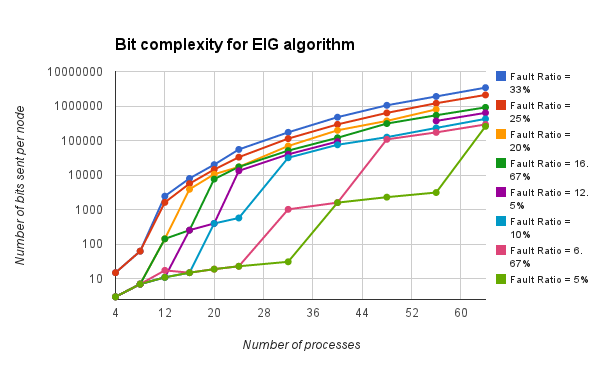
\includegraphics[scale=0.4]{eig}
\caption{Performance results for EIG algorithm (Log Scale)}
 \label{fig:eig}
\vspace{-2mm}
\end{figure}

%\begin{figure}[ht]
% \centering
%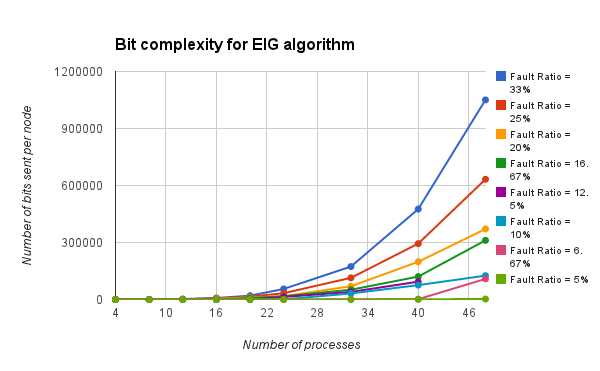
\includegraphics[scale=0.4]{eignolog}
%\caption{Consensus results for EIG algorithm}
% \label{fig:eignolog}
%\end{figure}
For the \textit{Pull-Push} algorithm, as the network size increases the bit complexity displays a poly-logarithmic growth. This can be seen in Fig. \ref{fig:pull_push}. The growth trend is similar for all fault ratios for small and larger networks. The increase in number of faults has an effect on the number of bits sent per process but only by a constant factor. This can be attributed to the fact that in the protocol, even if byzantine processes try to send conflicting values and a large number of them to samplers for the purpose of flooding, the samplers do not receive enough of them to forward these messages further in the protocol. Also note that for networks with $logn$ remaining the same, the bits sent per process is the same and it only changes at network sizes that are powers of $2$. This is because good processes only communicate with samplers of size $logn$. Hence, for larger networks, increasing the size of the network by less than $100\%$ will not affect the bandwidth consumption.
\begin{figure}[ht]
 \centering
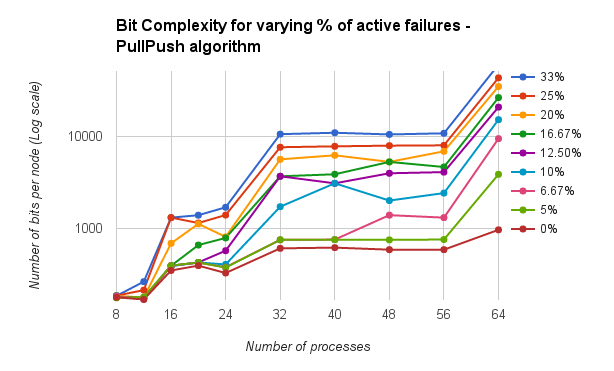
\includegraphics[scale=0.4]{pull_push}
\caption{Performance results for Pull-Push algorithm (Log scale)}
 \label{fig:pull_push}
\vspace{-2mm}
\end{figure}

From Figure \ref{fig:quorum}, algorithm \textit{Quorum} shows very high bits per process communication even for small networks. It increases rapidly as the network size increases. The reason for this is that \textit{Graded broadcast} requires all-to-all communication between processes and the protocol requires processes to run a deterministic byzantine agreement protocol for every subset of a committee in Stage $2$ of the protocol. The fault ratios do not have much of an effect on the communication costs. Byzantine processes are unable to increase bits on the network by participating in more sub-protocols than the algorithm requires since membership in a sub-protocol is dictated by their ID, which is fixed. Hence, more number of processes are unable to influence the communication cost greatly which is already high.  
\begin{figure}[ht]
 \centering
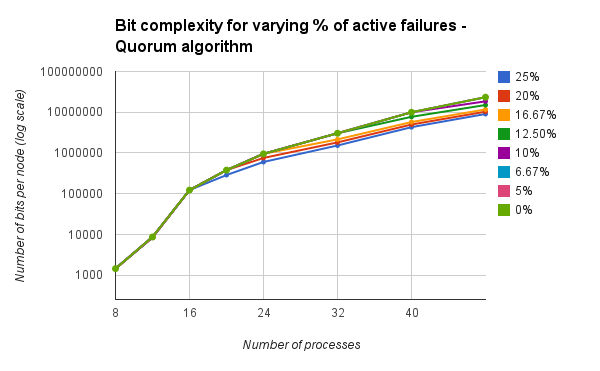
\includegraphics[scale=0.4]{quorum}
\caption{Performance results for Quorum algorithm (Log scale)}
 \label{fig:quorum}
\vspace{-2mm}
\end{figure}

Each of our algorithms for every configuration was run multiple times. In the analysis, each data point is an average over $5$ independent runs and we obtained confidence intervals for each of them. The confidence interval for algorithm \textit{Pull-Push} was $\pm 1\%$, for algorithm \textit{EIG} - $\pm 0.1\%$, and $\pm 0.5\%$ for algorithm \textit{Quorum}.

\subsection{Comparison}
For large networks ($n > 64$), we vary the ratio of faults to the number of processes ($f/n$), which lies in the range $[0, 1/3)$ for algorithms \textit{EIG} and \textit{Pull-Push}, and in the range $[0, 1/4)$ for algorithm \textit{Quorum}.
        As can be seen from Fig. \ref{fig:comp}, the algorithm \textit{Pull-Push} performs much better than the other algorithms for any fault percentage.

        Next, we modify the \textit{EIG} protocol a little to require that instead of sending the complete byzantine list every time, from round $4$ onwards only the changes to this list be sent in every round. We are motivated to do so since sending information about the existence of a process in the suspected byzantine list of another process in every round seems redundant. This does not change the correctness of the algorithm since all the good processes send the same changes to every other process in a round and in the next round the confirmation mechanism would confirm these updated lists. The rest of the algorithm works in the same way. Even though this does not change the communication complexity in the worst case, it overall reduces the communication bits as good processes would send a bit for every suspected byzantine process only in any one of the rounds instead of every round. This modified version of the algorithm performs much better. For small ratios, since the number of rounds is small, the number of bits sent per process remains the same. But, as the ratio increases, it varies greatly from the performance of algorithm \textit{EIG}.
\begin{figure}[ht]
 \centering
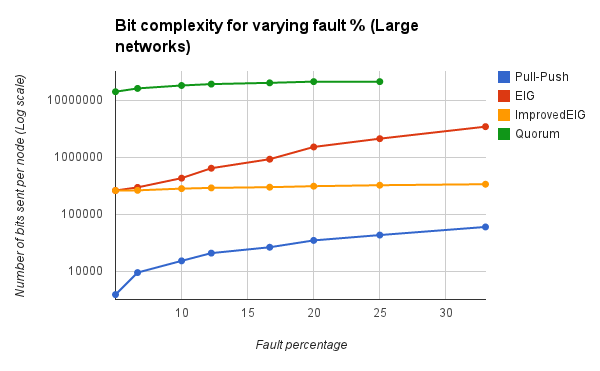
\includegraphics[scale=0.4]{LargeNetBit}
\caption{Comparison for large networks}
 \label{fig:comp}
\vspace{-2mm}
\end{figure}

\begin{figure}[ht]
 \centering
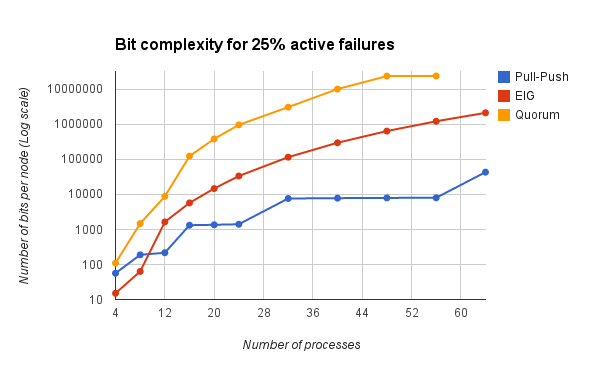
\includegraphics[scale=0.4]{Fault25}
\caption{Comparison for high \% of faults}
 \label{fig:fault25}
\vspace{-2mm}
\end{figure}

\begin{figure}[ht]
 \centering
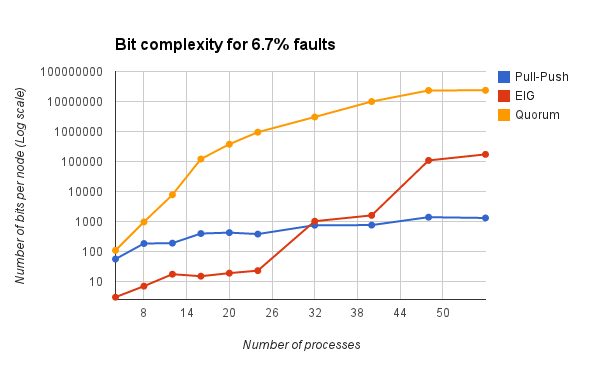
\includegraphics[scale=0.4]{Fault667}
\caption{Comparison for low \% of faults}
 \label{fig:fault667}
\vspace{-2mm}
\end{figure}

\begin{figure}[ht]
 \centering
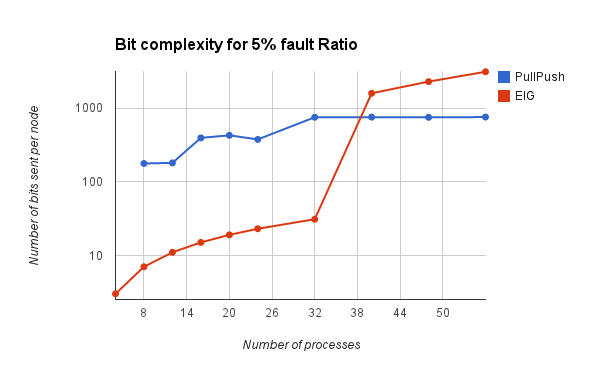
\includegraphics[scale=0.4]{Fault5}
\caption{Comparison for low \% of faults}
 \label{fig:fault5}
\vspace{-2mm}
\end{figure}

For small networks ($n < 40$), if the fault ratio is small and in the range $[0, 1/15)$, Figs. \ref{fig:fault667} and \ref{fig:fault5} show that algorithm \textit{EIG} performs much better than any of the other algorithms. This is simply because only the first three rounds of this algorithm will be executed and since the ratio is small, a simple broadcast is sufficient to gather all the information. \textit{Pull-Push} and \textit{Quorum}, which are more complex algorithms, perform worse in such scenarios. Fig. \ref{fig:fault25} shows that for higher fault ratios and any network size, algorithm \textit{Pull-Push} performs better.

    Depending on the system requirements such as how fast we want the information to reach the destination, bandwidth and so on, there were two mechanisms we used to send the messages. In an algorithm like \textit{Pull-Push}, where multiple message packets may be sent to the same process by a process in the same round, one could marshal all the packets into one packet and then send it. This obviously comes at the cost of parallelization where one has to first wait to receive all the messages from the previous round, perform operations and then send out messages all at once. While the number of messages sent per process changed when using the latter method, the number of bits sent remained the same.

%The difference in the number of messages sent for the two mechanisms can be seen in Fig. \ref{fig:opt}.
%\begin{figure}[h]
% \centering
%\includegraphics[scale=0.55]{optimized}
%\caption{ EIG algorithm when messages are grouped before sending}
% \label{fig:opt}
%\end{figure}

\subsection{Round Complexity}
Round complexity is the number of phases that have to be executed sequentially by a process and cannot be parallelized. For example, in algorithm \textit{EIG}, a round consists of broadcast of messages at the same level $i$ in the \textit{EIG} tree of each process. For algorithm \textit{Quorum}, a round consists of broadcast of messages during a particular sub-protocol. There are two ways to analyze the round complexity of this algorithm. The first is that each of the sub-protocols $S_i^j$ could be executed in parallel since none of these sub-protocols are dependent on each other. Hence, all of them together make one round. But, if parallel execution of these sub-protocols is not possible due to resource constraints then each of them is an independent round. We implemented the algorithm to run the sub-protocols in parallel since that improved the round complexity. For algorithm \textit{Pull-Push}, the push phase makes one round and sending, routing and answering in the pull phase form independent rounds.

\begin{figure}[ht]
 \centering
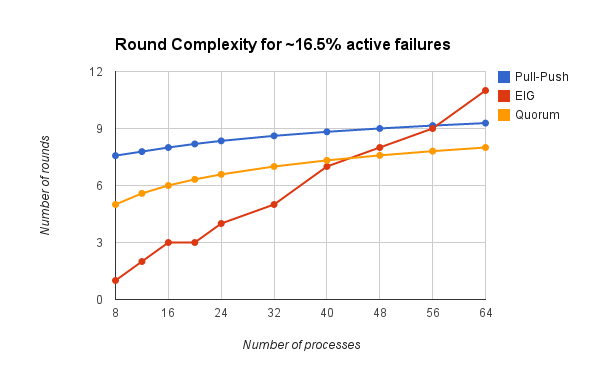
\includegraphics[scale=0.4]{Round16}
\caption{Round Complexity comparison}
 \label{fig:round16}
\vspace{-2mm}
\end{figure}

\begin{figure}[ht]
 \centering
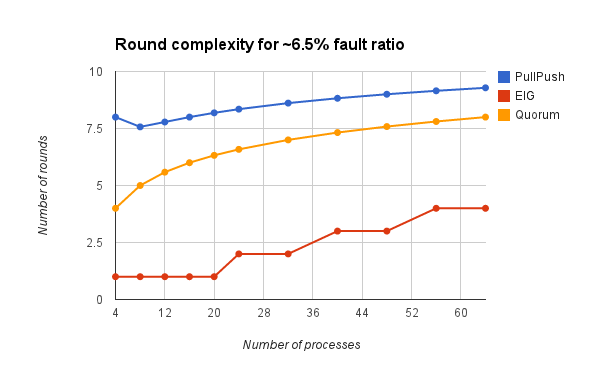
\includegraphics[scale=0.4]{Round6}
\caption{Round Complexity comparison}
 \label{fig:round6}
\vspace{-2mm}
\end{figure}

A comparison of the round complexities can be seen in Figs. \ref{fig:round16} and \ref{fig:round6} for fault percentage $~16.5\%$ and $~6.5\%$, respectively. We can see that for a very small ratio of $~6.5\%$ the round complexity of \textit{EIG} is better but for larger ratios and larger networks $(n > 40)$ \textit{Quorum} performs better than the other two. 


\subsection{Latency}

For performance comparison of latency, we compare the total CPU times and elapsed real time.  The total CPU time is the sum of CPU time consumed by all of the CPUs utilized by an execution of an algorithm. If a program has parallel tasks, the total CPU time takes into account the time taken by each of the tasks. Elapsed real time is simply the time taken from the start of a computer program until it terminates as measured by an ordinary clock. From Figures \ref{fig:cpu} and \ref{fig:elapsed}, we see that CPU time utilization and elapsed real time of \textit{EIG} increases rapidly and it is a lot slower compared to the other two algorithms. If we look at the elapsed real time, we can see that algorithm \textit{Quorum} remains the fastest throughout. This is because \textit{Quorum} is highly parallel. The trade-off here is that the CPU time utilization of \textit{Quorum} is a lot more than that of \textit{Pull-Push}. This trend is maintained for all fault ratios.

\begin{figure}[ht]
 \centering
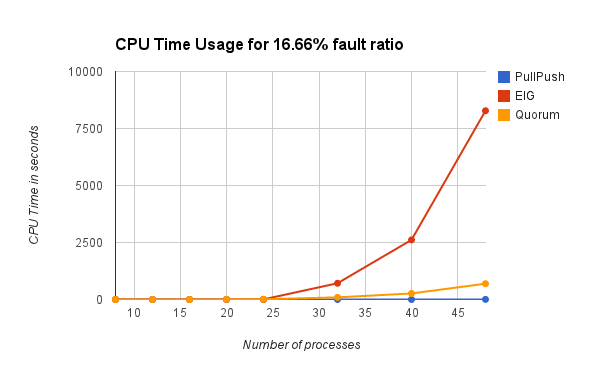
\includegraphics[scale=0.4]{cpu16}
\caption{CPU time utilization comparison}
 \label{fig:cpu}
\vspace{-2mm}
\end{figure}

\begin{figure}[ht]
 \centering
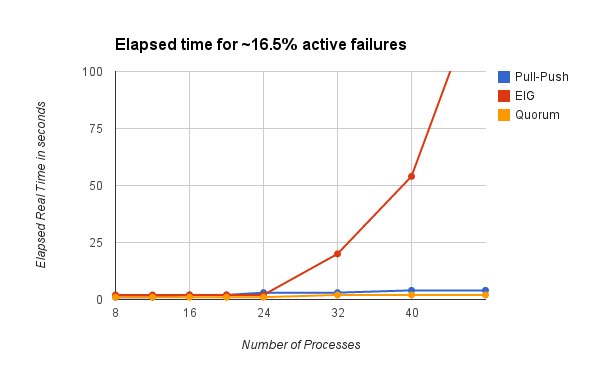
\includegraphics[scale=0.4]{elapsed16}
\caption{Elapsed real time comparison}
 \label{fig:elapsed}
\vspace{-2mm}
\end{figure}

%Fig. \ref{fig:time} the first mechanism for calculating time complexity of algorithm Quorum is used, where it is considered that all the subprotocols together form one round. This figure shows the algorithm Quorum gives better performance than algorithms EIG and Pull-Push as the number of processes in the network increases. Also, algorithm Pull-Push diverges in complexity due to increasing number of candidate strings that could be injected by the adversarial processes.

%Fig. \ref{fig:time_nopar}, shows a comparison of time complexities if each subprotocol in algorithm Quorum is treated as an individual round. In contrast to Fig. \ref{fig:time}, this figure clearly shows that the time complexity of algorithm Quorum increases rapidly, whereas for algorithms EIG and Pull-Push there is no drastic increase. Hence, if resources are limited and parallel processing of each subprotocol is not possible, algorithm Quorum does not give good performance.
%
%\begin{figure}[h]
% \centering
%\includegraphics[scale=0.55]{time_nopar}
%\caption{Time Complexity comparison no parallel execution}
% \label{fig:time_nopar}
%\end{figure}





\subsection{Discussion}

As can be seen from the results above, according to the requirements and resources available, each algorithm performs differently. The first thing to consider before implementation is what resources are available and how can a system be designed to obtain optimal results for the available resources. Implementing the testbed framework on a cluster allowed us to create realistic scenarios. We considered different byzantine behaviors for each algorithm and its consequences. To report on the number of bits sent per process in the worst case, we considered byzantine processes that try to flood the network. In this scenario, among the three algorithms we considered, algorithm \textit{Pull-Push} performs the best generally. However, in the case of a small network with number of processes less than $32$ and a low fault percentage - approximately less than $10\%$, algorithm \textit{EIG} performs better since it considers the number of faults in its protocol. 

If we were to consider a network with its size showing high variance over time, algorithm \textit{Pull-Push} has the advantage that the number of bits sent per node remains the same if the increase in size is within the next power of $2$. For strict bandwidth constraints, this allows high flexibility to change the size of the network. On the other hand, if we were to look at networks which did not change in size but had varying fault ratios, algorithm \textit{Quorum} inhibited a varying number of byzantine processes from changing the communication complexity much. This, however, is restricted to networks with high bandwidth in the first place. Our modified version of algorithm \textit{EIG} showed this characteristic as well. The number of bits sent per node increased very minimally on increasing the fault ratio and also performed much better when compared to \textit{Quorum} or \textit{EIG} as can be seen in Figure ~\ref{fig:comp}.

Furthermore, the implementation results demonstrated the trade-off between the number of communication bits and the number of rounds. Algorithm \textit{Quorum} terminated in lower number of rounds than \textit{Pull-Push} for all network sizes and fault ratios. This can be attributed to its highly parallel protocol. Algorithm \textit{EIG} displayed growth proportional to the size of the network, and performed well only for very low fault ratios of $<10\%$. These trends are reflected in the latency results as well when we compared the elapsed real time. However, the total CPU time utilization increased rapidly for \textit{Quorum} due to the exponential increase in the number of sub-protocols executed in parallel as the network size increased.

In the case of a denial of service attack, an increasing ratio of faulty processes reduced the communication overhead instead of increasing it. Crash failures also reported similar results. If the faulty processes sent out only arbitrary messages, the algorithms executed correctly without hampering the communication cost much when the ratio of byzantine processes was increased.

To further optimize the performance, one can improve certain tasks such as sending a larger message instead of many smaller messages or executing parallel tasks on multi-core machines. Another optimization that would have improved the running time of the system would be to use UDP connections instead of TCP since they take up less resources and provide lower overhead. Even though UDP connections do not guarantee message delivery, for a small system it could still be considered highly reliable. The rationale behind using TCP connections for our testbed framework was to model and understand implementation issues for more realistic distributed systems, which could have peers separated by geographical distance, requiring greater reliability. 

An analysis of the three algorithms and their performance for a wide range of number of processes and faults shows that communication of each process with fewer number of processes yields good results instead of all-to-all communication. This inhibits byzantine processes from influencing values of too many good processes. It is also important that requests from byzantine processes be throttled at an early stage. The good performance of the deterministic algorithm for small fault ratios shows that it is important to consider this factor when designing an algorithm.  Communication between multiple sets of quorums allows parallel tasks to be executed and gives good latency results. The combined use of these techniques would help design improved algorithms to solve the problem of distributed consensus. 



\section{Conclusion}
\label{sec:conc}
In real-world systems, achieving distributed consensus has become increasingly important. In most cases, consensus is a small but frequently used sub-component of a larger protocol such as in state machine replication protocols or in distributed databases. Thus, understanding the performance of algorithms for various scenarios occurring in real-time is essential to the overall performance of such systems. One needs to consider implementation issues that come along with any of these algorithms and not only their theoretical results. 

In this paper, we focused on implementation and analysis of three recently proposed algorithms with best results for their respective agendas. An Exponential Information Gathering protocol for consensus \cite{KM13} (algorithm \textit{EIG}) showed that deterministic algorithms have come a long way since the early results. We further improved upon the results obtained for this algorithm. In general the randomized algorithm \textit{Pull-Push} \cite{BGH13}, performed better than the other two in terms of communication complexity. When latency was considered, as can be seen in Fig. \ref{fig:elapsed}, algorithm \textit{Quorum} \cite{BPV06} performed better. In real-time situations, as the number of processes in a network increase the probability of having faulty processes in the network naturally increases. Hence, even though algorithm \textit{EIG} shows better performance when the fault ratio is small, under high fault ratio the performance degrades. Quantifying the performance of the algorithms empirically provides a
practical understanding of how the different algorithms perform under
different situations to achieve consensus in distributed systems.


\newpage
\bibliographystyle{plainnat}
\bibliography{bibliography}

\newpage
\appendix
\section{Appendix}
\label{sec:appendix}

\subsection{Algorithm Quorum\cite{BPV06}}

\begin{definition}
A protocol $P$ is said to achieve graded broadcast if, at the beginning of the protocol the dealer $D$ holds a value $v$, and at the end of the protocol, every process $P_i$ outputs a pair $(v_i, c_i)$ where $c_i \in \{0, 1, 2\}$ denotes the confidence of the process in value $v_i$. With that, the following properties should hold:
\vspace{-2mm}
\begin{enumerate}
\item If $D$ is honest, then $v_i = v$ and $c_i = 2$ for every honest process $P_i$. 
\item For any two honest processes $P_i$ and $P_j$, $\mid c_i - c_j \mid \leq 1$.
\item (Consistency) For any two honest processes $P_i$ and $P_j$, if $c_i > 0$ and $c_j > 0$, then $v_i = v_j$.
\end{enumerate}
\end{definition}

The graded broadcast algorithm is described in detail as follows: \\
\textbf{Input to the Dealer $D$:} A value $v$  \\
\textbf{Output of process $P_i$:} A pair $(v_i, c_i)$ \\
\textbf{Step 1} The dealer $D$ distributes $v$ to all the processes. \\
\textbf{Step 2} (For every process $P_i$) Send $v_i$, the received value from the dealer, to all other processes.  \\
\textbf{Step 3} (For every process $P_j$) Let $v_i^j$ denote the message from process $P_i$ in Step 2. If there is a value $\mu$ such that $\geq n - k$ of the $v_i^j$'s are equal to $\mu$, then send $\mu$ to all the processes. Else, send $\bot$. \\
\textbf{Step 4} (For every process $P_i$) Let $\mathtt{num}_\mu$ denote the number of players that sent $\mu$ to $P_i$ in Step 3. \\
\vspace{-4mm}
\begin{itemize}
\item If $\mathtt{num}_\mu \geq 2k + 1$ for some $\mu$, output $(\mu, 2)$.
\item If $2k \geq \mathtt{num}_\mu \geq k + 1$ for some $\mu$, output $(\mu, 1)$.
\item If $\mathtt{num}_\mu \leq k $ for all $\mu$, output $(\bot, 0)$.
\end{itemize}

\subsection{Algorithm Pull-Push \cite{BGH13}}



        \begin{minipage}[h]{0.90\columnwidth}
        \begingroup
        \removelatexerror
        \begin{algorithm}[H]
         \caption{Push phase}%
         \footnotesize
               \label{alg:push}%
      %\SetAlgoLined
               \KwIn{Process $P_i$ with a random string $g_{string}$, a list of all strings $C_{string}$}
        \KwOut{Each node creates a candidate strings list $L_{P_i}$}
        
        $g_{string} \gets$ createRandString()\;

        broadcast$(g_{string})$\;

        $L_{P_i} \gets g_{string}$\;

        
        \ForEach{ $str \in C_{string}$}{

            $I_{str} \gets$ getPushQuorum($\mathtt{str}, P_i$)\;
            \ForEach{$p \in I_{str}$}{
                \If{$recv(I_s) == str$}{
                    $num++$\;
                }
            }
            \If{$\mathtt{num} > len(I_s)$}{
                $L_{P_i} \gets L_{P_i} \cup s$\;
            }

        }


    \end{algorithm}%
    \endgroup
  \end{minipage}%


\begin{minipage}[H]{0.90\columnwidth}
    \begin{Ualgorithm}
         \footnotesize
         \caption{Sending Pull Request}%
               \label{alg:send_pull}%
      %\SetAlgoLined
               \KwIn{$L_{P_i}$, list of candidates for node $P_i$}
        \KwOut{String agreed upon}
        
        
        \ForEach{ $s \in L_{P_i}$}{
            $r_{P_i, s} \gets$ generateRand()\;
            $J_{r,s} \gets$ getPollList($r_{P_i, s}, P_i$)\;
            $H_s \gets$ getPullQuorum($s$, $P_i$)\;
            send$(POLL, s, r_{P_i, s}, J_{r,s})$\;
            send$(PULL, s, r_{P_i, s}, H_s)$\;

            Upon event: recv$(ANSWER,s,r)  \Leftarrow w$\;
            \Indp 
                \If{$w \in J_{r,s}$}{
                    $\mathtt{count}_s ++$\;
                    \If{$\mathtt{count}_s > \frac{1}{2}|J_{r,s}|$}{
                        has\_decided $\gets$ true\;
                        $\mathtt{final}_s \gets s$\;
                        \Return{$s$}\;
                    }
                }
        }
    \end{Ualgorithm}%
  \end{minipage}%




        \begin{minipage}[H]{0.90\columnwidth}
        \begingroup
        \removelatexerror
        \begin{algorithm}[H]
         \caption{Routing Pull Request}%
    \footnotesize
               \label{alg:rout_pull}%
      %\SetAlgoLined
        Upon event: $\mathtt{recv}(PULL, s, r_{x, s}, H_s) \Leftarrow x$\;
        \Indp 
            \If{$(g_{string} == s)$ and $(P_i \in H_s)$}{
                $J_{x,r_{x,s}} \gets$ getPollList($r_{x, s}, x$)\;
                \ForEach{$w \in J_{x,r_{x,s}}$}{
                    $H_{w,s} \gets$ getPullQuorum($s$, $w$)\;
                    send$(ROUTE, x, s, r_{x, s}, w) \Rightarrow H_{w,s}$\;
                }
            }
        \Indm Upon event: $\mathtt{recv}(ROUTE, x, s, r_{x,s}, w) \Leftarrow P_j$\;
        \Indp 
            $H_{x,s} \gets$ getPullQuorum($s$, $x$)\;
            $J_{x,r_{x,s}} \gets$ getPollList($r_{x, s}, x$)\;
            \If{$(g_{string} == s)$ and $(P_j \in H_{x,s})$ and $(w \in J_{x,r_{x,s}})$}{
                $\mathtt{fw\_count}_{s,x}++$\;
                \If{$\mathtt{fw\_count}_{s,x} > \frac{1}{2}|H_{x,s}|$}{
                    send$(FORWARD, x, s, r_{x, s}) \Rightarrow w$\;
                    $\mathtt{fw\_count}_{s,x} \gets \infty$\;
                }
            }


    \end{algorithm}%
    \endgroup
  \end{minipage}%





        \begin{minipage}[H]{0.90\columnwidth}
        \begingroup
        \removelatexerror
        \begin{algorithm}[H]
         \footnotesize
         \caption{Answering Pull Request}%
               \label{alg:ans_pull}%
      %\SetAlgoLined
        Upon event: $\mathtt{recv}(ROUTE, x, s, r_{x, s}) \Leftarrow z$\;
        \Indp 
            \If{$\mathtt{count}_s > \mathtt{log}^2n$}{
                Wait for has\_decided\;
            }
            $J_{x,r_{x,s}} \gets$ getPollList($r_{x, s}, x$)\;
            $H_{P_i,s} \gets$ getPullQuorum($s$, $P_i$)\;
            \If{$(g_{string} == s)$ and $(P_i \in J_{x, r_{x,s}})$ and $(z \in H(P_i, s))$}{
                $\mathtt{fw\_count}_{s,x}++$\;
                \If{$(\mathtt{fw\_count}_{s,x} > \frac{1}{2}|H_{x,s}|)$ and $((x, s) \in \mathtt{Polled})$}{
                    $\mathtt{count}_s ++$\;
                    send$(ANSWER, s, r_{x, s}) \Rightarrow x$\;
                }
            }
        \Indm Upon event: $\mathtt{recv}(POLL, s, r_{x,s}) \Leftarrow x$\;
        \Indp 
            $J_{x,r_{x,s}} \gets$ getPollList($r_{x, s}, x$)\;
            \If{$P_i \in J_{x, r_{x,s}}$}{
                $\mathtt{Polled} \gets \mathtt{Polled} \cup (x,s)$\;
                \If{$\mathtt{fw\_count}_{s,x} > \frac{1}{2}|H_{x,s}|$}{
                    $\mathtt{count}_s ++$\;
                    send$(ANSWER, s, r_{x, s}) \Rightarrow x$\;
                    $\mathtt{fw\_count}_{s,x} \gets \infty$\;
                }
            }

    \end{algorithm}%
    \endgroup
  \end{minipage}%


%\begin{enumerate}
%\item Sending Queries: Each node $x$ verifies each string $s \in L_x$ by polling a set of nodes. A random string $r_{x,s}$ is chosen to define $J(x, r_{x,s})$. A different random string is used for each candidate string $s$. Next, $x$ sends a `POLL' request to Poll List $J(x, r_{x,s})$ and a `PULL' request to Push Quorum $H(x, s)$.
%\item Answering: 
%\begin{enumerate}
%\item A node $y \in H(x, s)$ forwards a request received from $x$ iff $s$ is its initial candidate string $s_y$. The request is forwarded to nodes in $J(x, r_x)$ routed through their Pull Quorums by sending a `ROUTE' request.
%\item A node $z$ in the Pull Quorum of $w \in J(x, R_x)$ ($z \in H(s, w)$) forwards the request to $w$ iff $s = s_z$ and $z$ received the request from more than half of the nodes of $H(x, s)$. 
%\item Finally, a node $w \in J(x, r_x)$ replies to a `PULL' request from $x$ if:
%\begin{itemize}
%\item the pull request was received from a majority of $H(w, s)$;
%\item either one of its pull requests was answered (thus $w$ knows $g_{\mathtt{string}}$), and $s_w$ was changed accordingly;
%\item or it currently has received less than $log^2n$ pull requests. 
%\end{itemize}
%\end{enumerate}
%\item Deciding: If $x$ receives answers from a majority of nodes in $J(x, r_{x,s})$, $s$ is deemed to be the global string.
%\end{enumerate}



\end{document}
